\chapter{Технологическая часть}

В данной части приведены средства реализации, особенности реализации алгоритмов и функциональные тесты.

\section{Средства реализации}

Программа реализована на языке \texttt{C++} (стандарт C++17)~\cite{cpp_standard}.
Для сборки используется компилятор \texttt{g++} (GCC)~\cite{gcc}.
При реализации многопоточности применяются стандартные средства библиотеки \texttt{C++}: \texttt{std::thread} и механизмы синхронизации, предусмотренные стандартом~\cite{cpp_standard}.

\section{Реализация алгоритмов}

В вычислительном этапе (ОУ2) реализованы два варианта поиска компонент связности:
\begin{itemize}
	\item последовательный алгоритм на основе обхода графа в ширину (BFS);
	\item параллельный алгоритм на основе структуры непересекающихся множеств (DSU) с использованием $k$ вспомогательных потоков.
\end{itemize}

Листинг последовательного алгоритма приведён в приложении на листинге~\ref{lst:cc_seq}, параллельного алгоритма --- на листинге~\ref{lst:cc_par}.

\subsection{Последовательный алгоритм (BFS)}

Для каждого ещё не размеченного узла запускается обход в ширину, при котором все достижимые вершины получают одинаковый идентификатор компоненты.
Для обхода используется очередь (\texttt{std::queue}), а для эффективного доступа к соседям предварительно строится список смежности \texttt{adj}.
Результатом работы алгоритма является массив идентификаторов компонент \texttt{comp\_id} и количество компонент \texttt{comp\_count}.

\subsection{Параллельный алгоритм (DSU, $k$ потоков)}

Параллельный вариант выполняет объединение вершин по рёбрам графа с использованием DSU.
Список рёбер разбивается на $k$ частей, и каждая часть обрабатывается отдельным потоком: для каждого ребра выполняется операция \texttt{unite}.
После завершения потоков выполняется построение массива \texttt{comp\_id}: каждой вершине назначается номер компоненты на основе её корня DSU.
Для корректной работы в многопоточной среде используется потокобезопасная реализация DSU.

\section{Функциональные тесты}

Функциональные тесты направлены на проверку корректности разбиения графа на компоненты связности.
Набор тестов приведён в таблице~\ref{tab:func_tests_cc}.

\begin{table}[H]
\centering
\small
\setlength{\tabcolsep}{3pt}
\renewcommand{\arraystretch}{1.15}
\caption{Функциональные тесты поиска компонент связности}
\label{tab:func_tests_cc}
\begin{tabularx}{\linewidth}{|c|>{\raggedright\arraybackslash}X|>{\raggedright\arraybackslash}X|>{\raggedright\arraybackslash}X|}
\hline
\textbf{№} & \textbf{Входные данные (граф)} & \textbf{Ожидаемый результат} & \textbf{Проверяемое} \\
\hline
1 & $n=0,\; E=\varnothing$ &
$\textit{comp\_count}=0,\; \textit{comp\_id}=\varnothing$ &
Граничный случай: пустой граф \\
\hline
2 & $n=1,\; E=\varnothing$ &
$\textit{comp\_count}=1,\; \textit{comp\_id}=[0]$ &
Одна вершина без рёбер \\
\hline
3 & $n=5,\; E=\varnothing$ &
$\textit{comp\_count}=5,\; \textit{comp\_id}=[0,1,2,3,4]$ (или эквивалентно) &
Граф без рёбер: каждая вершина отдельная компонента \\
\hline
4 & $n=5,\; E=\{(0,1),(1,2),(2,3),(3,4)\}$ &
$\textit{comp\_count}=1$, все вершины в одной компоненте &
Связный граф (цепочка) \\
\hline
5 & $n=6,\; E=\{(0,1),(1,2),(3,4)\}$ &
$\textit{comp\_count}=3$: $\{0,1,2\}$ вместе, $\{3,4\}$ вместе, $\{5\}$ отдельно &
Несколько компонент + изолированная вершина \\
\hline
6 & $n=6,\; E=\{(0,1),(1,2),(2,0),(3,4),(4,5),(5,3)\}$ &
$\textit{comp\_count}=2$: $\{0,1,2\}$ и $\{3,4,5\}$ &
Компоненты с циклами \\
\hline
7 & $n=4,\; E=\{(0,1),(1,2),(2,3),(0,2)\}$ &
$\textit{comp\_count}=1$ &
Наличие «лишних» рёбер не меняет компоненту \\
\hline
8 & $n=5$, $E$ содержит некорректные рёбра: $(0,1),(-1,2),(2,10)$ &
Компоненты определяются только корректными рёбрами: $(0,1)$ соединяет 0 и 1, остальные вершины изолированы &
Игнорирование некорректных вершин в рёбрах \\
\hline
9 & Один и тот же граф как в тесте 5, запуск обоих алгоритмов &
Разбиение на компоненты эквивалентно (с точностью до переименования идентификаторов) &
Согласованность результатов BFS и DSU \\
\hline
10 & Один и тот же граф, запуск DSU при $k\le 0$ и при $k=1$ &
Результат одинаковый по разбиению на компоненты &
Нормализация параметра $k$ (минимум 1) \\
\hline
\end{tabularx}
\end{table}


При сравнении результатов последовательного и параллельного алгоритмов учитывается, что номера компонент могут отличаться.
Корректность сравнения проверяется по отношению эквивалентности: для любых вершин $i$ и $j$ должно выполняться, что они принадлежат одной компоненте в первом результате тогда и только тогда, когда они принадлежат одной компоненте во втором результате.

\section{Демонстрация работы программы}

На рисунке~\ref{fig:demo_components} показан пример результата работы программы: граф разбит на компоненты связности, после чего каждая компонента окрашена в отдельный цвет и сохранена в выходной \texttt{dot}-файл.
Демонстрация соответствует дополнительному этапу ОУ+ (ЛР8), формирующему \texttt{dot}-файл для визуализации.

\begin{figure}[H]
	\centering
	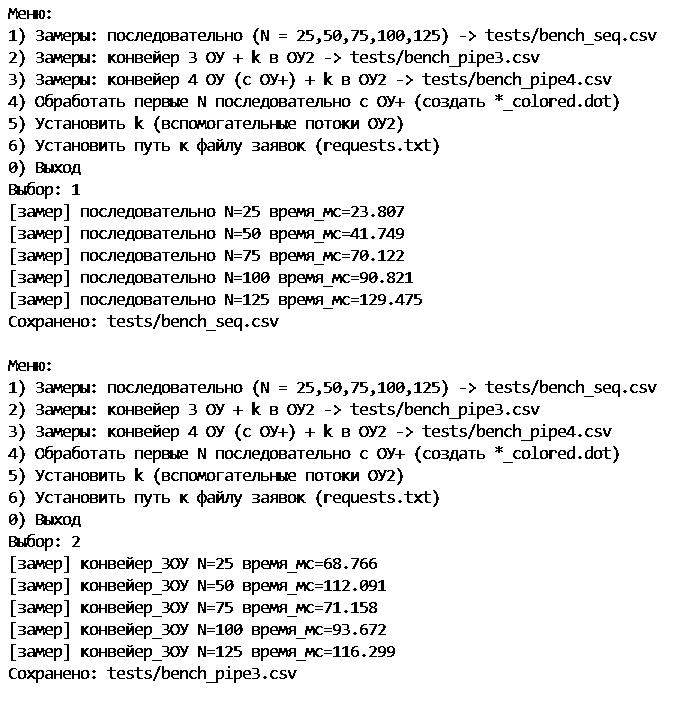
\includegraphics[width=0.9\linewidth]{images/image1.png}
	\caption{Пример визуализации компонент связности (одна компонента --- один цвет)}
	\label{fig:demo_components}
\end{figure}
